\section{Beamline}

The CLAS12 beamline is made up of several pieces, each discussed below. The positioning and composition of the beamline
depends on the run configuration, that can be:

\begin{itemize}
	\item FTOn: Forward Tagger present and operational. The Moller shield starts at z=877 mm from the target center to.
	\item FTOff: FT is present but not operational. The FT tracker is replaced by shielding.
                 The Moller shield starts at z=430 mm from the target center, and additional shielding is present to connect it to the FT.
\end{itemize}


\begin{figure}
	\centering
	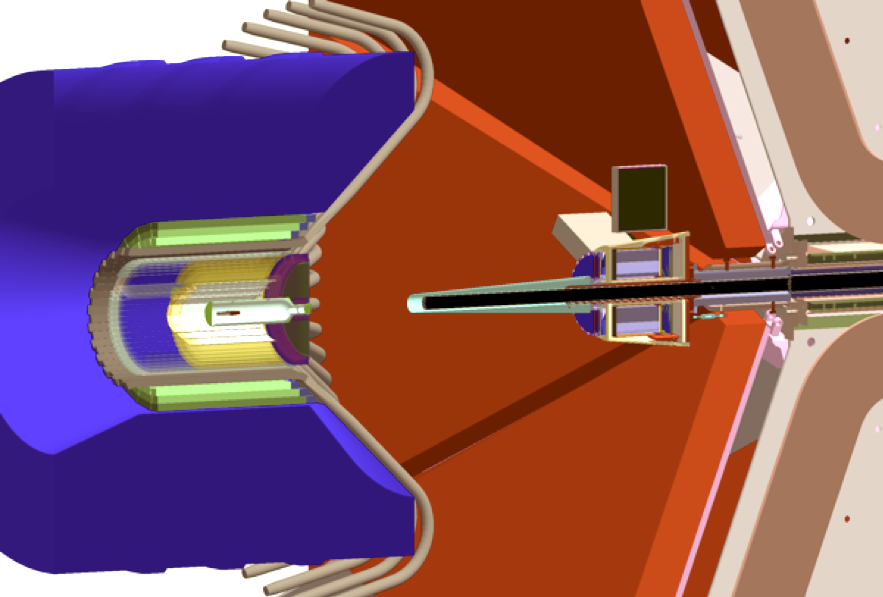
\includegraphics[width=0.98\columnwidth,keepaspectratio]{img/ftOnGeometry.png}
	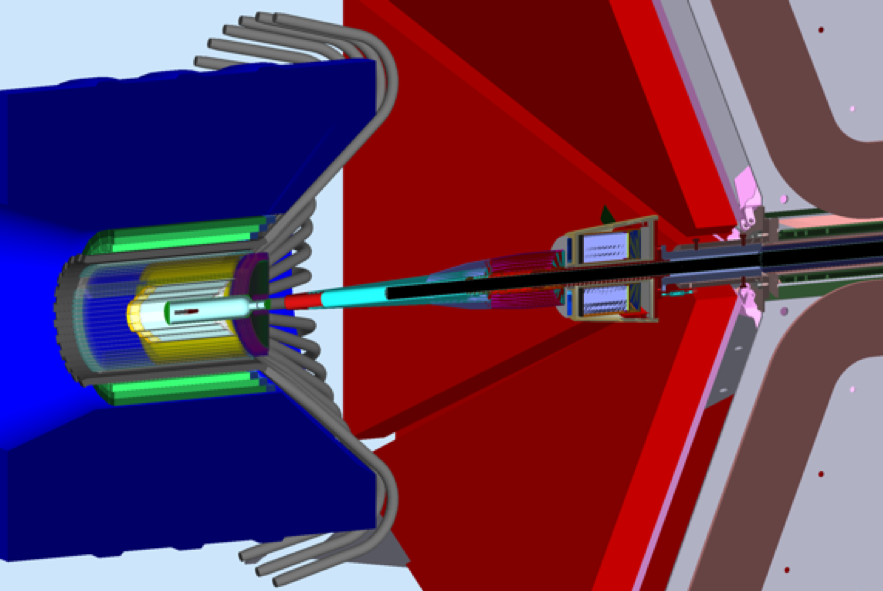
\includegraphics[width=0.98\columnwidth,keepaspectratio]{img/ftOffGeometry.png}
   \caption{The two possible CLAS12 configurations. Top: FTOn. To clear its acceptance at forward angles ($2.50-4.50$ degrees)
            the Moller shield (cyan color) is attached to the FT tracker, starting at $z=877$ mm from the target.
            Bottom: FToff; the FT is present but not operational. The FT tracker is replaced with a shield.
            The Moller cone is placed at $z=430$ mm from the target and additional shielding minimize background in Region 1 Drift Chambers.}
	\label{fig:beamlineGeometry}
\end{figure}

\subsection{Vacuum pipe}

A stainless steel vacuum pipes that contain the eletron beam. The pipe starts downstream of the target at $z=80cm$
and changes dimensions inside the torus and downstream of the torus as detailed in Table \ref{tab:beampipe}

\begin{table}[h]
	\begin{center}
		\begin{tabular}{| c | c | c |}
			\hline \hline
			                & Thickness (mm) & Inner Radius (mm)   \\
			\hline
              Upstream      &    1.6     &    26.9 \\
              Inside        &    1.6     &    33.3 \\
            Downstream      &    3.2     &    60.3 \\
			\hline \hline
		\end{tabular}
	\end{center}
	\caption{The vacuum pipe three dimensions sets (in mm) upstream, inside and downstream of the torus}\label{tab:beampipe}
\end{table}


\subsection{Moeller Shielding}
The Moeller shielding is composed by the following elements, shown in \F{moellerShielding}

\begin{figure}
	\centering
	\includegraphics[width=0.98\columnwidth,keepaspectratio]{img/moellerShielding.png}
   \caption{The two possible CLAS12 configurations. Top: FTOn. To clear its acceptance at forward angles ($2.50-4.50$ degrees)
            the Moller shield (cyan color) is attached to the FT tracker, starting at $z=877$ mm from the target.
            Bottom: FToff; the FT is present but not operational. The FT tracker is replaced with a shield.
            The Moller cone is placed at $z=430$ mm from the target and additional shielding minimize background in Region 1 Drift Chambers.}
	\label{fig:moellerShielding}
\end{figure}


\begin{itemize}
\item FTOn: Forward Tagger present and operational. The Moller shield starts at z=877 mm from the target center to.
\item a Tungsten cone with increasing thickness.
\item
\item
\item
\item
\end{itemize}




\subsection{Torus Shielding}
shielding around the vacuum pipe inside the torus hub in the form of tungsten bricks

\subsection{Donwstream shielding}
shielding downstream of the torus in the form of a connecting tungsten nose and a long lead pipe.


There are two

\subsection{Geometry}

The beamline geometry is entirely imported from the engineering CAD model.


\subsubsection{Geometry Git Location}

